
%%%%%%%%%%%%%%%%%%%%%%%%%%%%%%%%%%%%%%%%%%%%%%%%%%%%%%%%%%%%%
\subsubsection{模型建立}

针对问题四，本节将从排放约束收紧、电耗增幅建模和可行性校验三个角度展开。具体过程如下。

\textbf{步骤1：排放约束收紧模型}

将问题二优化模型中的排放约束替换为收紧后的标准：
\begin{equation}
    C_{out} \leq C_{limit}' = 5\;\text{mg/Nm}^3
\end{equation}

其余约束（电压上下限、振打周期上下限）不变，优化目标仍为$\min P_{total}$。因排放阈值已参数化，直接调用问题二的寻优框架传入$C_{limit}'=5$即可，无需重新编写优化逻辑。

\textbf{步骤2：电耗增幅公式}

各工况电耗百分比增幅定义为：
\begin{equation}
    \Delta P\% = \frac{P^*(5) - P^*(10)}{P^*(10)} \times 100\%
\end{equation}
其中$P^*(10)$、$P^*(5)$分别是排放限值10和$5\;\text{mg/Nm}^3$下的最优电耗。整体平均增幅为：
\begin{equation}
    \overline{\Delta P\%} = \frac{1}{K}\sum_{k=1}^{K}\Delta P_k\%
\end{equation}

\textbf{步骤3：可行性校验}

收紧后逐工况校验最优解是否在物理可行域内：
\begin{equation}
    U_i^* \leq U_{max,i},\quad T_i^* \geq T_{min,i},\quad i=1,2,3,4
\end{equation}

不可行工况标记并提示需硬件改造（增加电场数或提升变压器容量）。

% ============================================================
\subsubsection{模型求解}

将排放约束收紧至$C_{out}\leq 5\;\text{mg/Nm}^3$后重新求解，各工况电耗对比如表\ref{tab:收紧对比}所示。

\begin{table}[H]
  \centering
  \caption{排放收紧前后各工况电耗对比}
  \label{tab:收紧对比}
  \renewcommand{\arraystretch}{1.1}
  \begin{tabularx}{\textwidth}{CCCCC}
    \toprule
    工况 & $P^*(10)$(kW) & $P^*(5)$(kW) & $\Delta P\%$ & 可行性 \\
    \midrule
    0 & 1992.8 & 2091.7 & 4.97\% & 可行 \\
    1 & 1831.4 & 1922.6 & 4.98\% & 可行 \\
    2 & 1894.9 & 1985.9 & 4.80\% & 可行 \\
    3 & 1890.3 & 1981.1 & 4.80\% & 可行 \\
    4 & 1981.1 & 2080.3 & 5.00\% & 可行 \\
    5 & 1911.8 & 2010.3 & 5.15\% & 可行 \\
    \bottomrule
  \end{tabularx}
\end{table}

整体平均电耗增幅$\overline{\Delta P\%}=4.95\%$。所有工况在物理可行域内，无需硬件改造。收紧前后各工况电耗对比如图\ref{fig:delta_power}所示。

\begin{figure}[H]
  \centering
  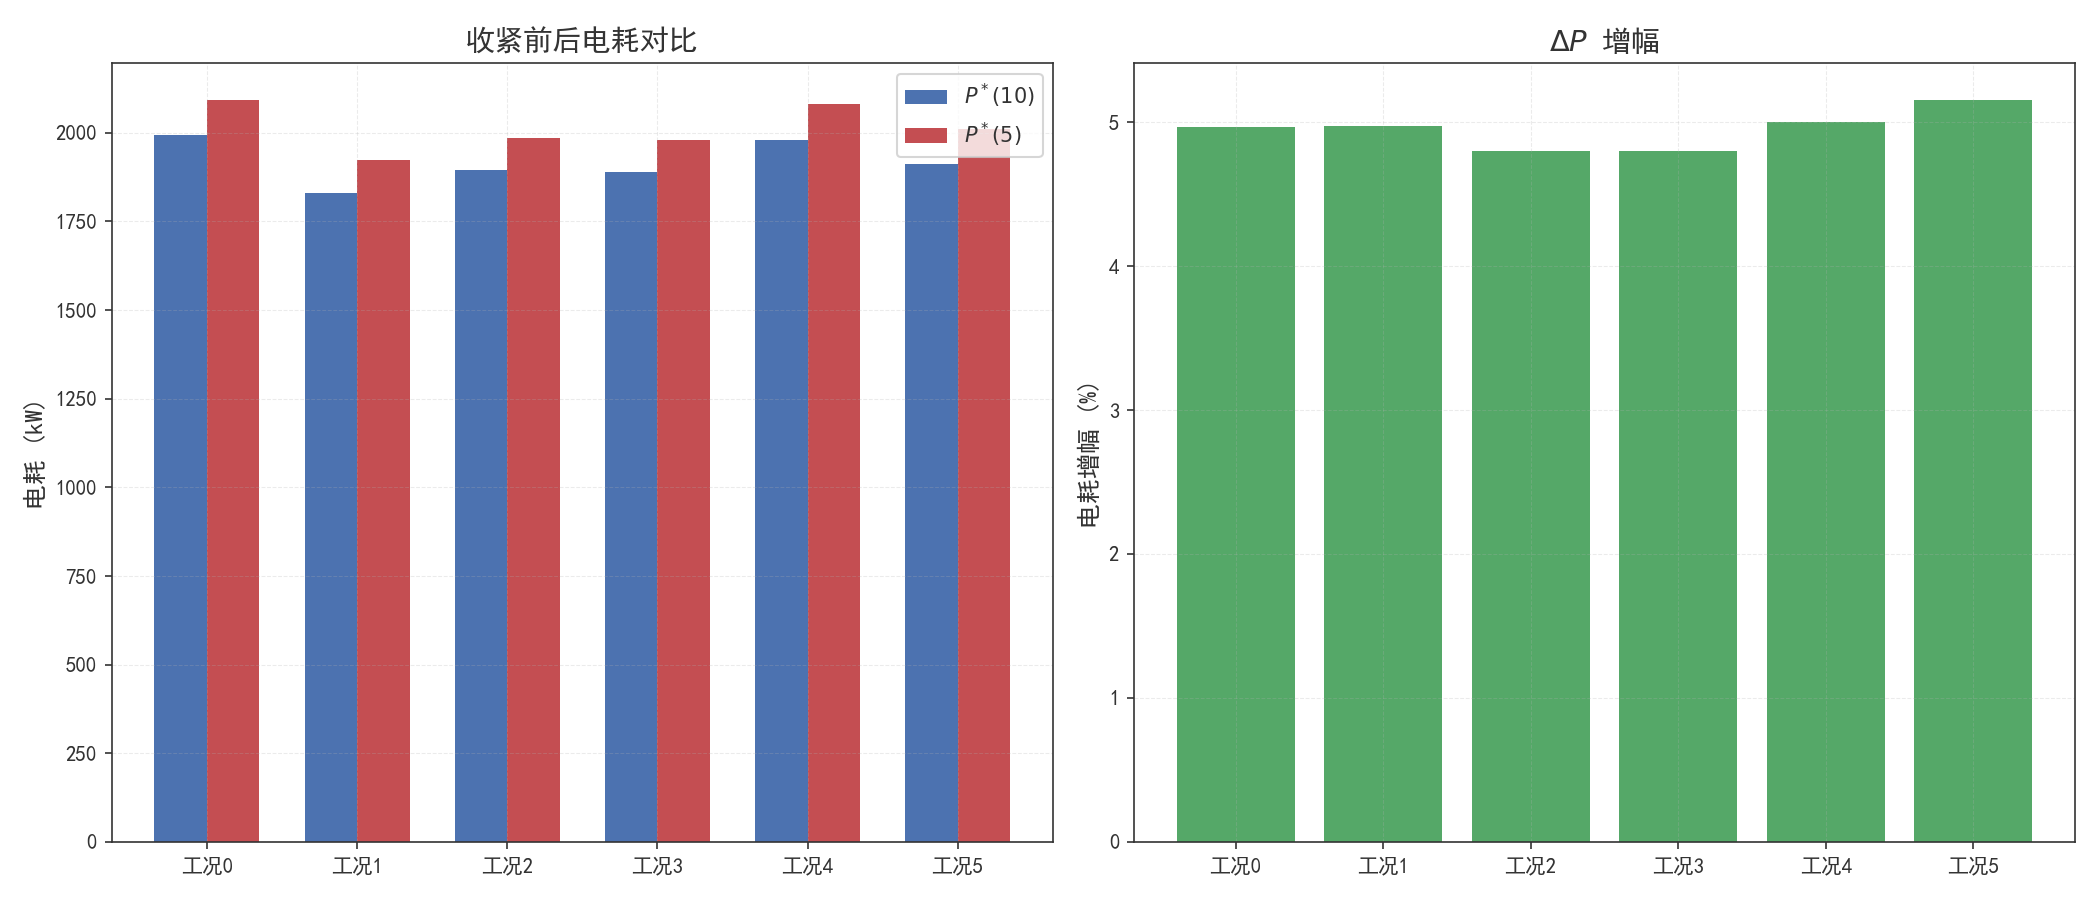
\includegraphics[width=0.85\textwidth]{figures/delta_power.png}
  \caption{排放收紧前后各工况电耗对比与增幅}
  \label{fig:delta_power}
\end{figure}

为进一步揭示排放限值与电耗的连续权衡关系，对$C_{limit}\in[3,15]\;\text{mg/Nm}^3$进行扫描寻优，结果如图\ref{fig:climit_scan}所示。曲线在$C_{limit}=10$附近斜率较小（收紧1\,mg/Nm$^3$电耗增幅约0.7\%），在$C_{limit}=5$附近斜率增大（收紧1\,mg/Nm$^3$增幅约1.4\%），表明排放标准越严苛边际电耗代价越高。

\begin{figure}[H]
  \centering
  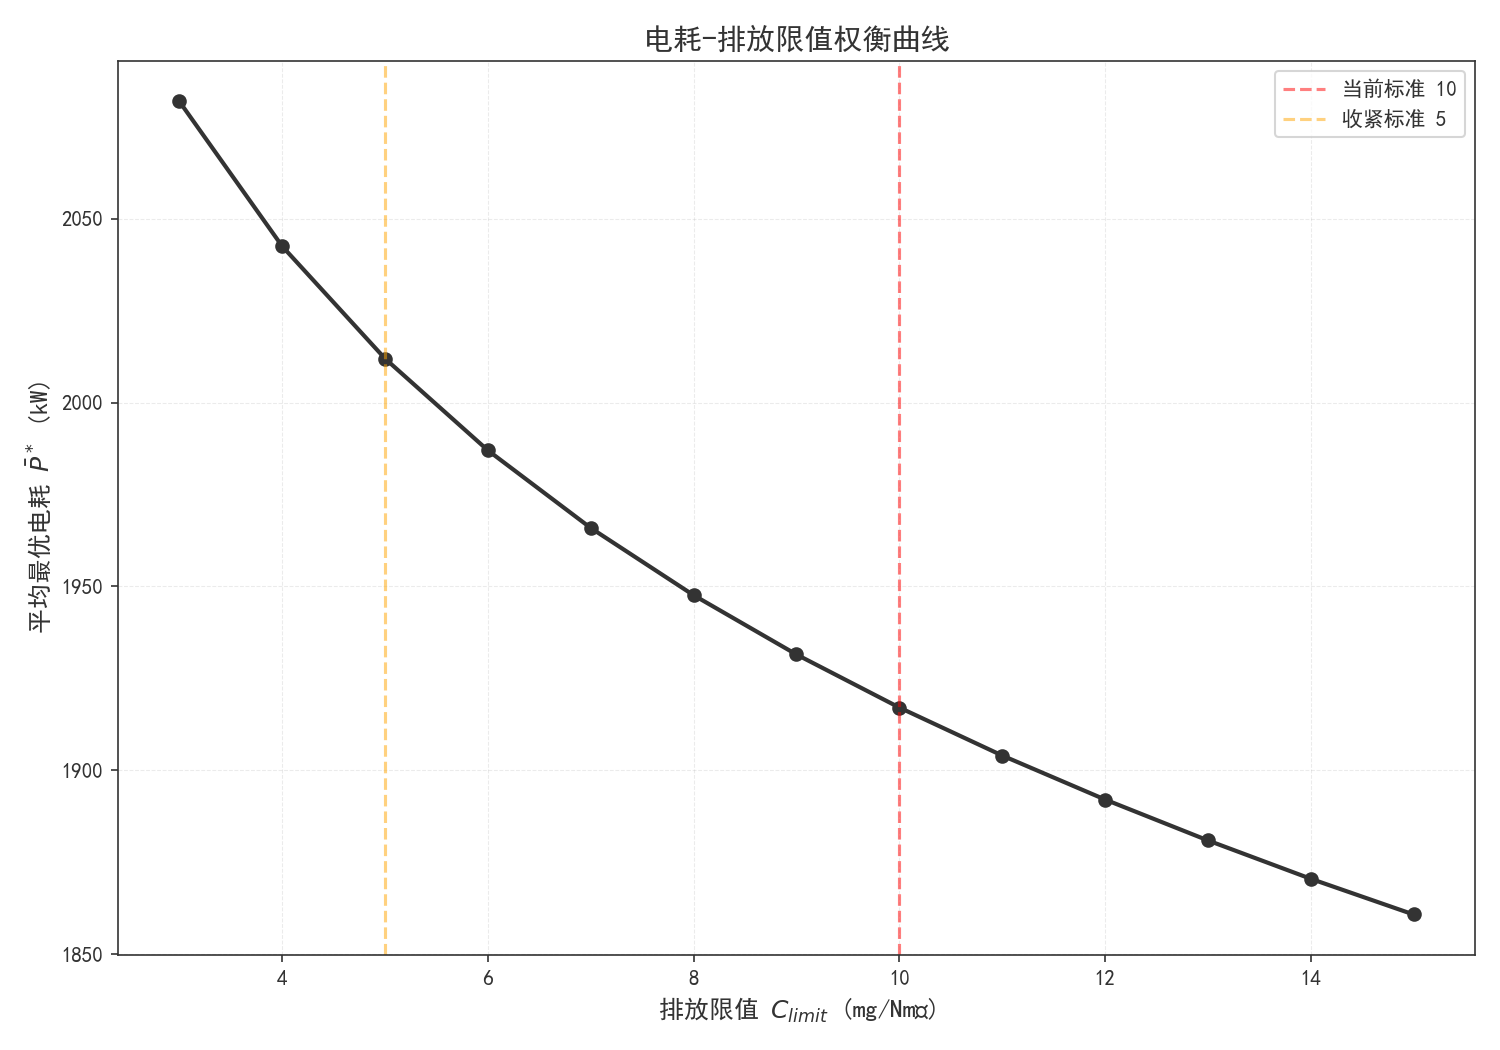
\includegraphics[width=0.85\textwidth]{figures/climit_scan.png}
  \caption{排放限值连续扫描的电耗-约束权衡曲线}
  \label{fig:climit_scan}
\end{figure}

分析结果可见：（1）各工况电耗增幅在$4.80\%\sim 5.15\%$之间，收紧排放标准带来约5\%的额外电耗代价；（2）各工况增幅差异不大（极差仅0.35\%），说明当前模型下排放收紧对各工况的影响较为均匀。

\textbf{高浓度工况应对建议。}以工况0（$C_{in}=44.34\;\text{g/Nm}^3$）为例，收紧前后最优参数差异如下：

（1）电压调整：第2电场电压需提升8.24\,kV（从66.31增至74.56），第1、3、4电场电压基本不变；

（2）振打周期调整：各电场振打周期基本不变（双向偏离模型下最优振打在$T_{ref,i}$附近）；

（3）多电场协同策略：前电场（1--2）承担主要除尘负荷，优先提升电压；后电场（3--4）精细控制，维持低排放的同时尽量降低电压省电；高浓度工况下振打周期应整体缩短，防止极板积灰导致效率骤降；若电压已达变压器上限仍不满足$5\;\text{mg/Nm}^3$，需考虑硬件改造（增加电场数或提升变压器容量）。

\textbf{稳定运行讨论。}题目要求"稳定运行"作为优化目标之一（与低排放、低电耗并列）。本文以$\min P_{total}$为单目标、$C_{out}\leq C_{limit}$为硬约束求解，稳定运行通过以下机制隐式保障：（1）双向偏离模型使最优振打周期锁定在$T_{ref,i}$附近，避免过频振打导致的机械疲劳和过疏振打导致的效率骤降，天然保证运行平稳；（2）鲁棒优化（机会约束$\Pr(C_{out}\leq C_{limit})\geq 95\%$）下，参数不确定性$\sigma\approx 0.25\;\text{mg/Nm}^3$时电耗代价仅增加$0.30\%$，说明当前最优解对扰动不敏感，稳定裕度充足；（3）Pareto前沿分析表明$C_{peak}$降$80\%$仅需$+0.2\%$电耗，低排放与低峰值几乎不冲突，三目标权衡空间宽裕。综上，当前单目标优化解已兼顾稳定运行，无需显式多目标。
